The analytical solution in Eq.~\eqref{eq:AnalyticSol} sheds a new light onto the
behaviour of the numerical neural network training. In order to study the
training process, the NNPDF collaboration has successfully developed so-called
{\em closure tests}. A closure test uses synthetic data, generated using a known
set of PDFs, to train the neural network. The PDFs used for generating the data
are called here {\em input}\ PDFs. The results of the training are then compared
to the known input PDFs; the performance of the training algorithm and the NN
architecture are assessed by quantifying the comparison between trained PDFs and
input PDFs. Following the original presentation in Ref.~\cite{NNPDF:2014otw}, we
distinguish three levels of closure tests, which are defined by the complexity
of the data used to train the NNs. We use the standard NNPDF nomenclature and
refer to these three levels as level-0 (L0), level-1 (L1), and level-2 (L2)
closure tests and we denote the input PDFs used to generate the data as $\fin$.

Let us start by discussing the case of L0 closure tests. In this case, the data are
given by
\begin{equation}
    \label{eq:DataL0}
    Y_I = T[\fin]_I
        = \sum_{i=1}^{\nflav} \sum_{\alpha=1}^{\ngrid} \FKtab_{Ii\alpha} \fin_{i\alpha}\, ,
\end{equation}
or equivalently, suppressing the indices,
\begin{equation}
    \label{eq:DataL0NoIndices}
    Y = \FKtab \fin\, .
\end{equation}
Using L0 data in the analytical expression for the trained network in
Eq.~\eqref{eq:AnalyticSol} allows a simplification of the second term,
\ldd{will type correct formulae here}
\begin{align}
    \label{eq:L0ClosureTrained}
    V(t) Y = \sumprime_{i} Z^{(i)} \left(1 - e^{-h^{(i)}t}\right)
        \sum_{k\in\perp} w^{(i)}_k \fin_k\, .
\end{align}
Interestingly, for $t\to\infty$,
\begin{align}
    \label{eq:L0ClosureInfiniteTraining}
    \lim_{t\to\infty} V(t) Y = \finperp\, ,
\end{align}
and therefore the $V$ component of the trained solution reproduces exactly the
component of the PDF that lies in  the subspace orthogonal to the kernel of
$\Theta$.

\ldd{we need to compute the the scalar product $(z^{k},f^\textin)$ for all values of 
$k$ at different training times between $t=0$ and $T_{\mathrm{ref}}=20,000$. We may be 
able to see explicitly that the eigenvectors of the NTK really align with the 'true' 
solution.}

Distance between the numerical minimization and the analytical formula as a
function of training time $t$

\ldd{Compute distances between numerical and analytical solutions using the
standard NNPDF definition of the distance. Same as the ones that are below, but
using L0 data}


\newpage


% ===================================
\begin{figure}[t!]
  \centering
  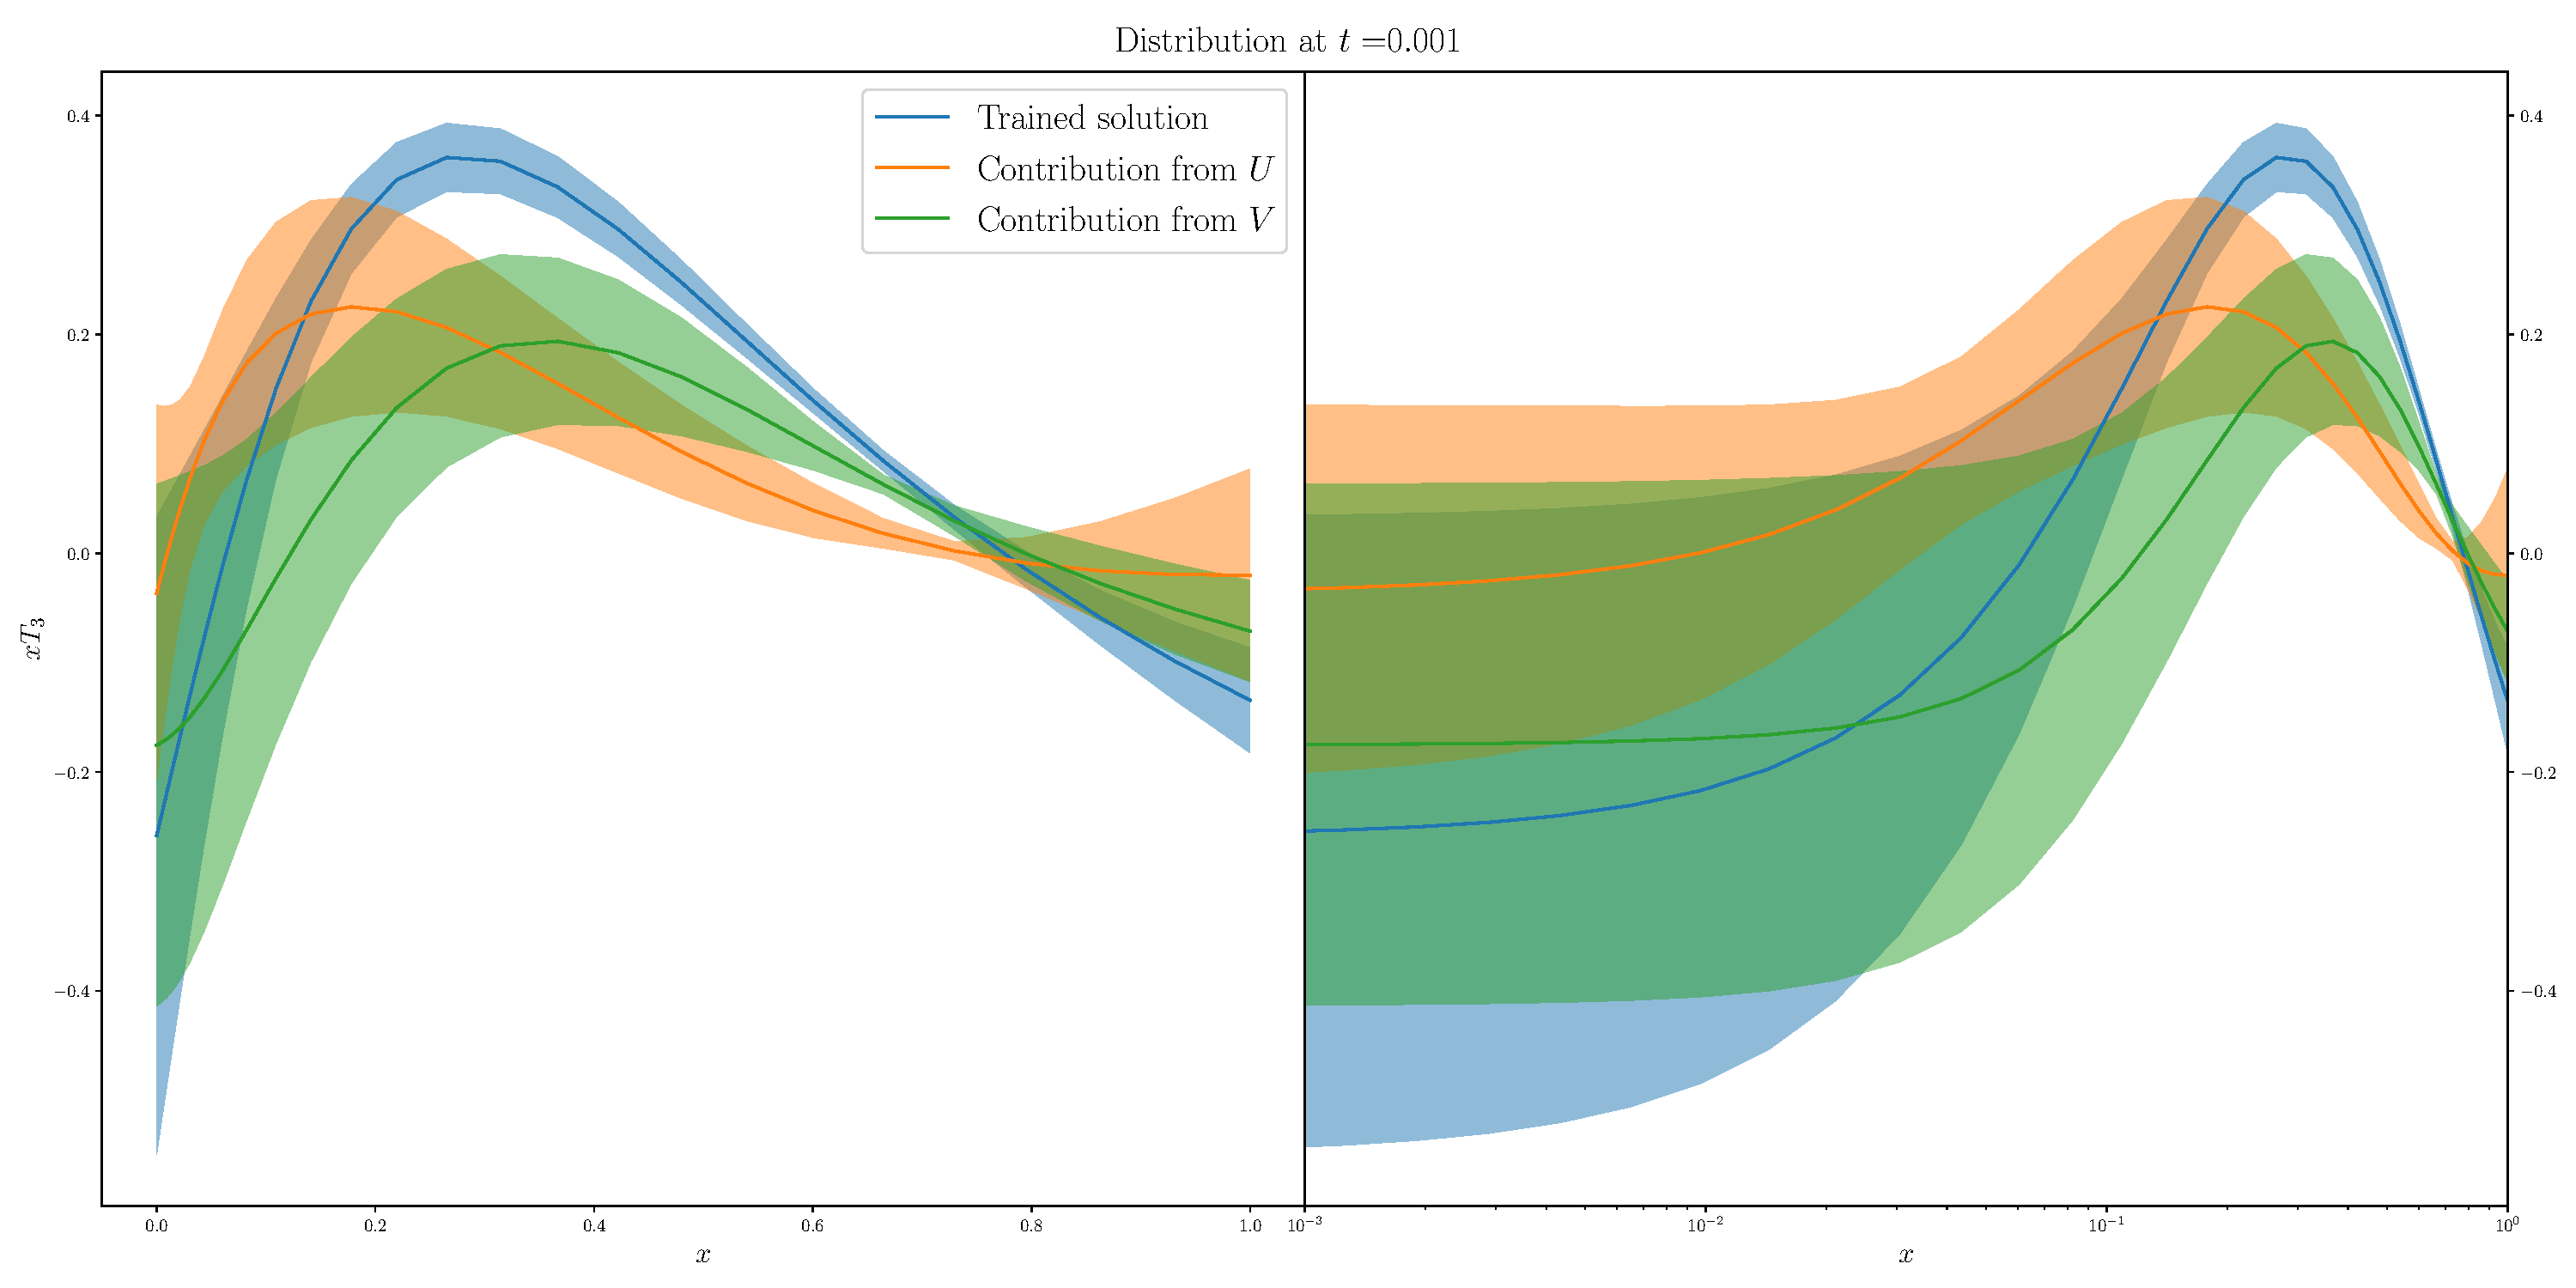
\includegraphics[width=0.65\textwidth]{plots/xT3_u_v_contribution_small_t.pdf}
  \\
  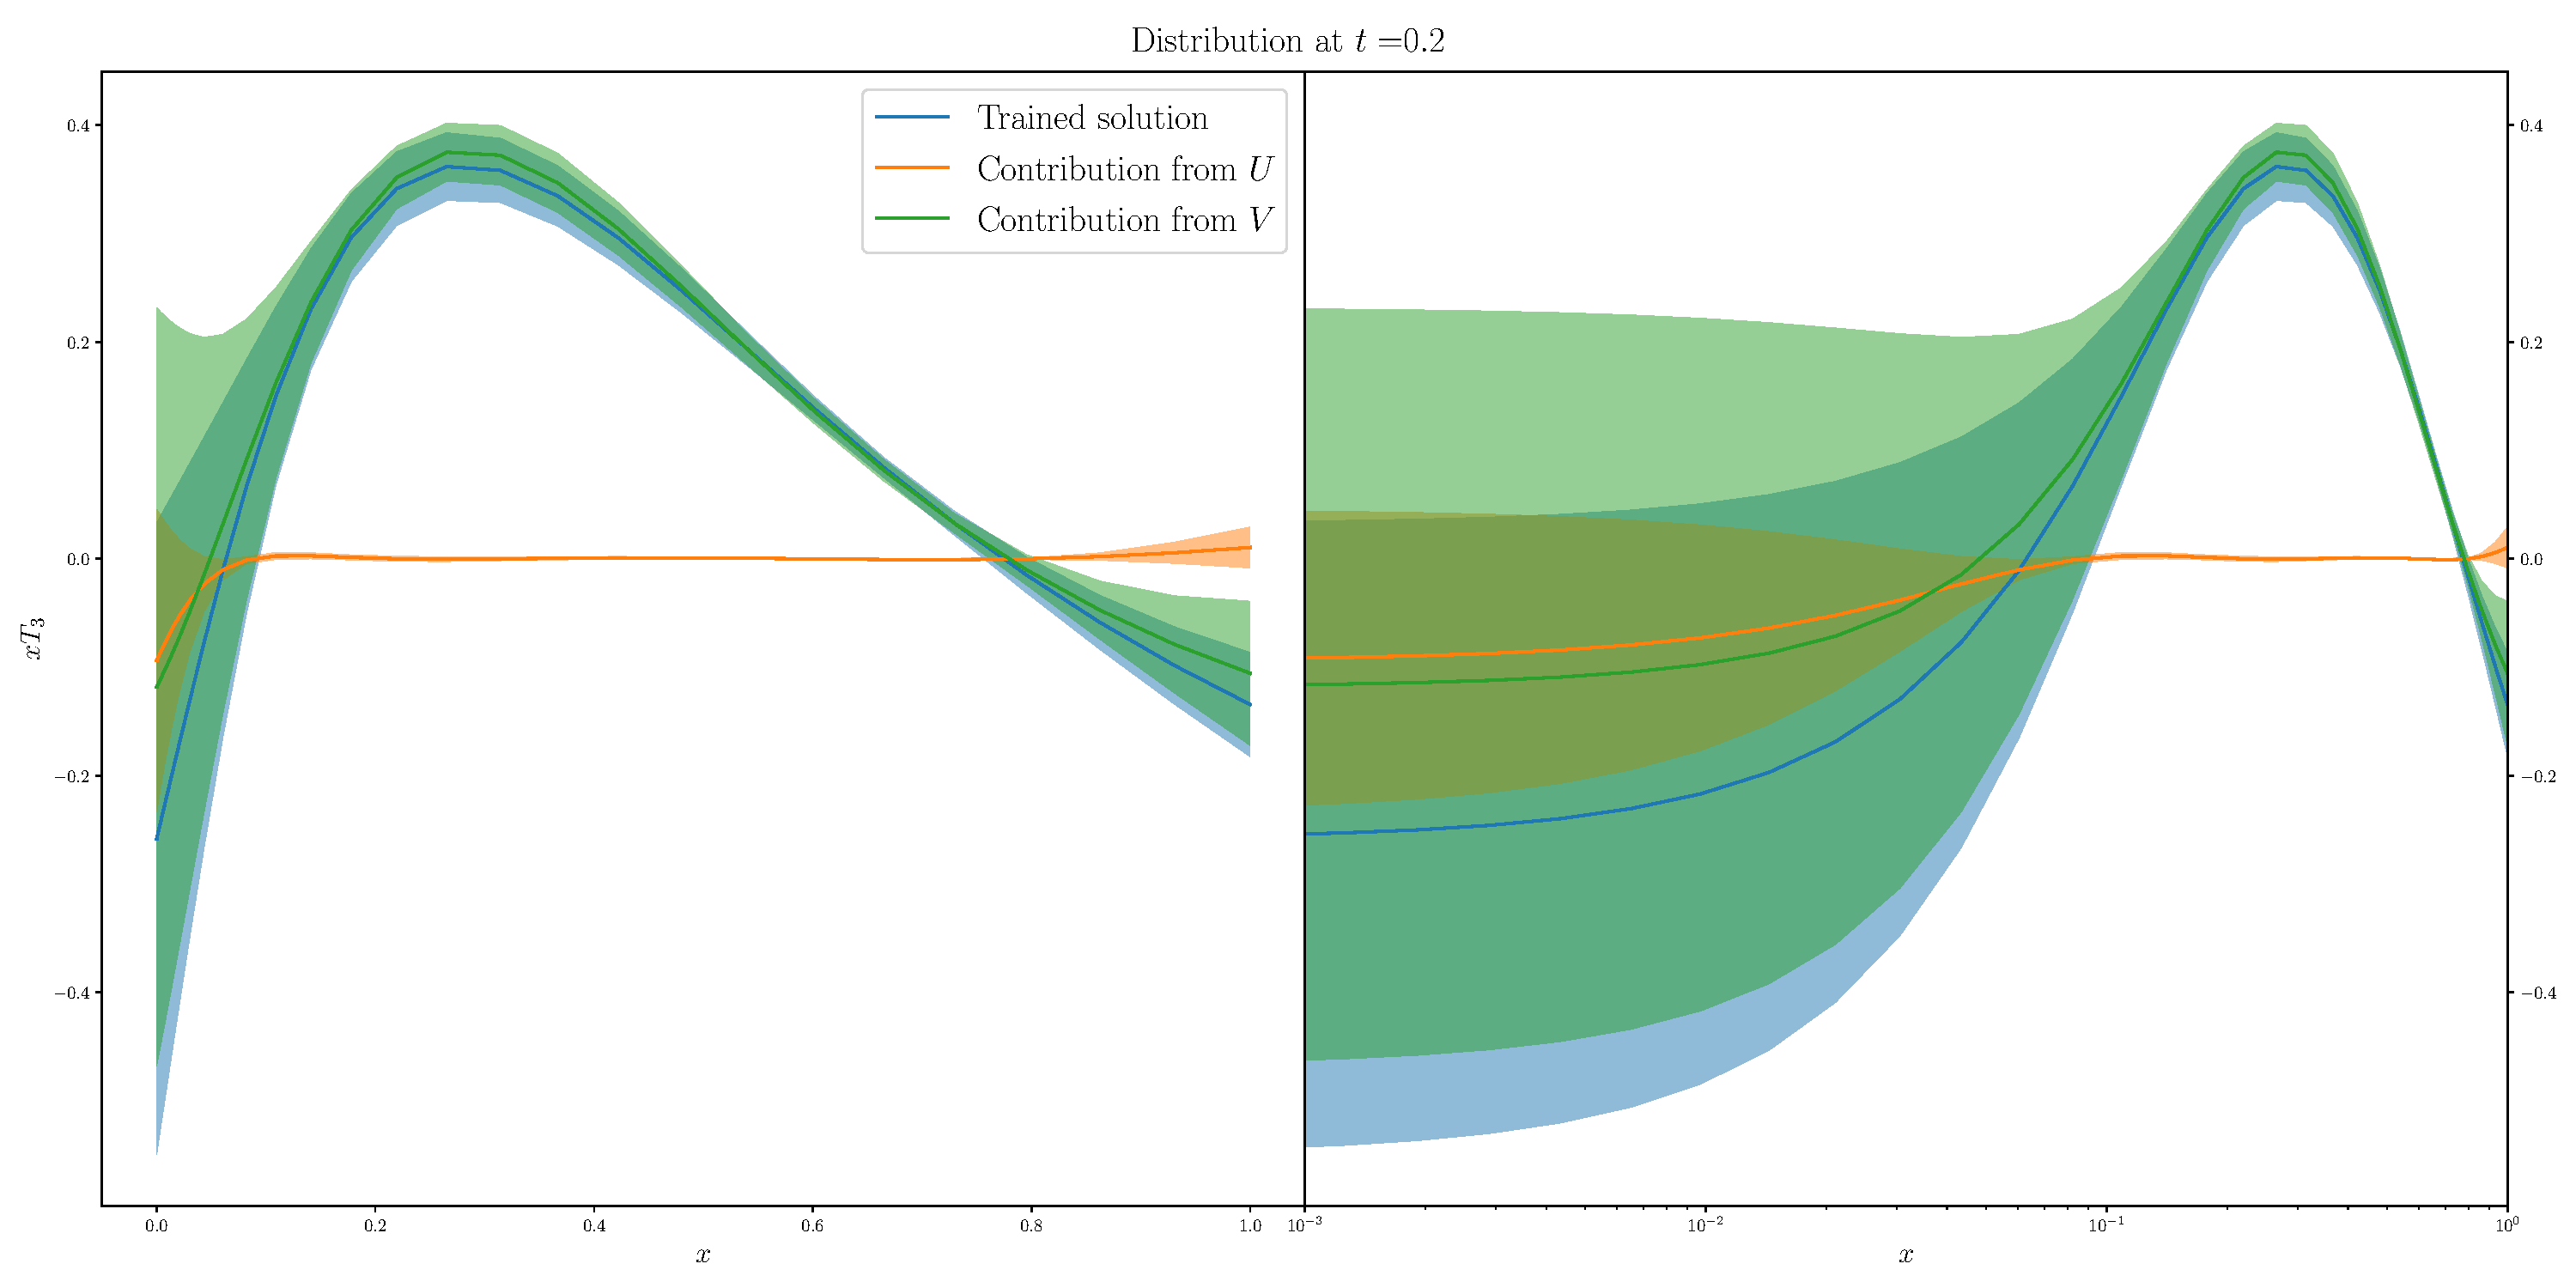
\includegraphics[width=0.65\textwidth]{plots/xT3_u_v_contribution_eot.pdf}
  \caption{Contribution of the $U$ and $V$ terms to the solution. The top panel
  shows this breakdown at early stages of the analytical training ($t=0.001$);
  the bottom panel shows the contributions at the end of training (eot) (same as
  Fig.~\ref{fig:xT3_analytical}). These plots have been obtained by taking the
  $t_{\rm ref} = 30000$ and $f_0 = f_{t_{\rm ref}}$ using L2 data. \ac{These
  plots will be modified (font size, etc...) to match the other figures.}}
\end{figure}
% ===================================

\begin{figure}[t!]
  \centering
  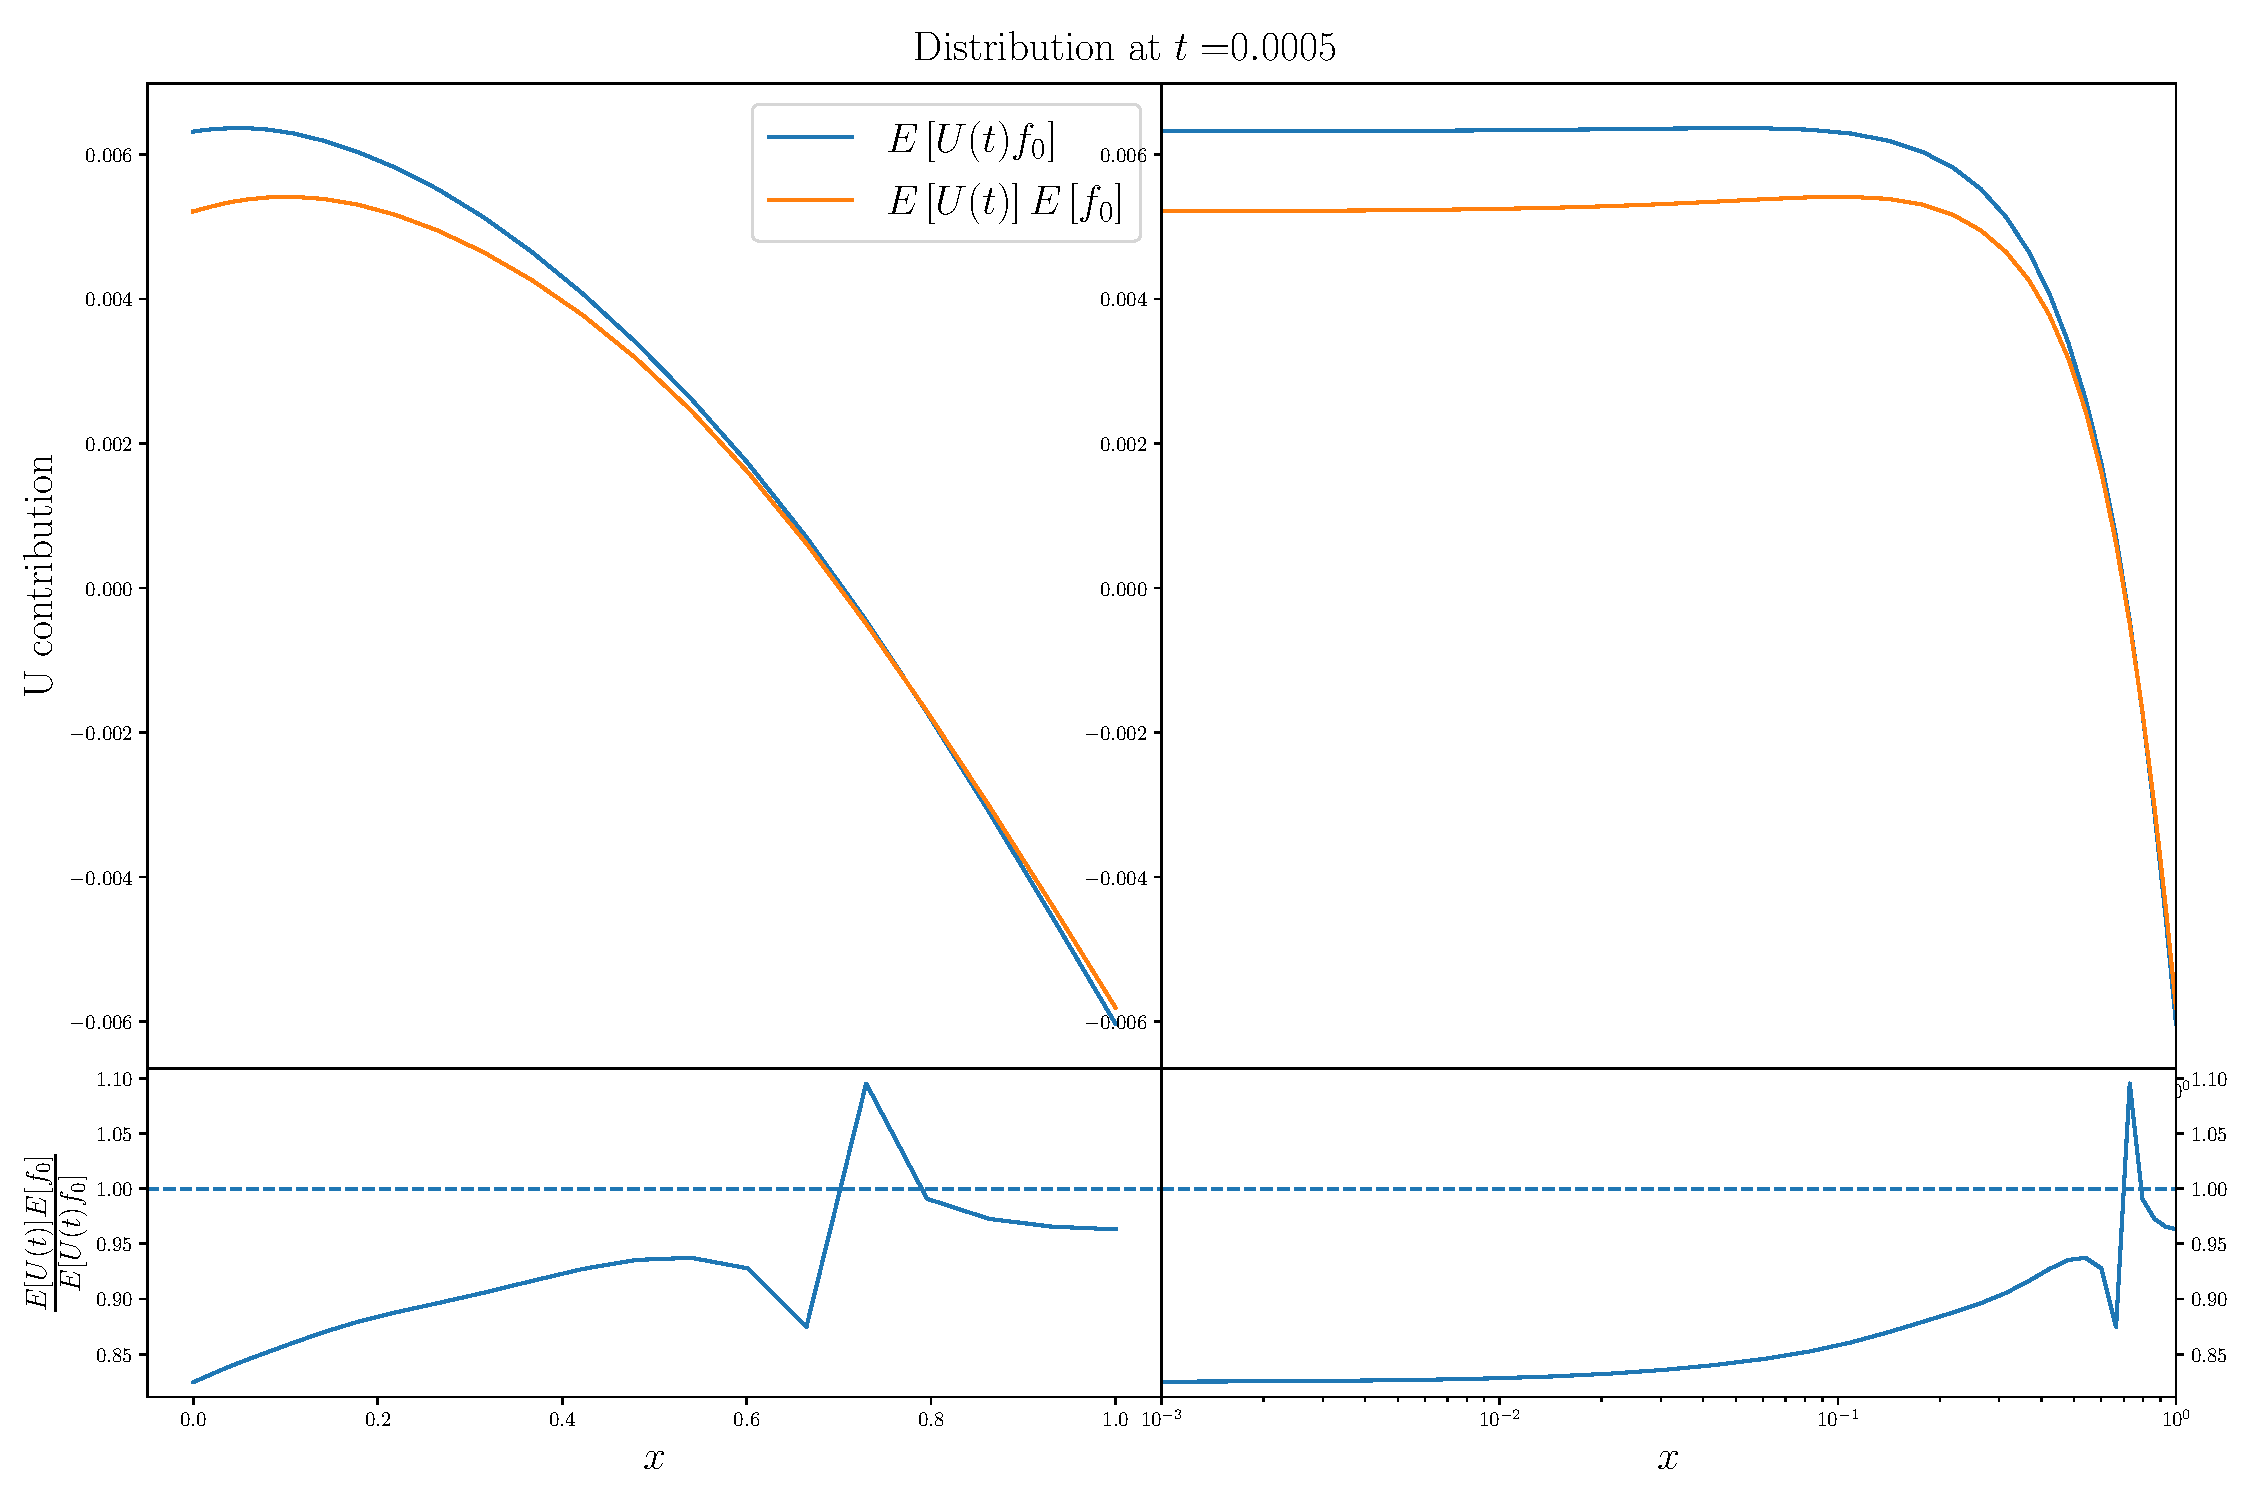
\includegraphics[width=0.65\textwidth]{plots/xT3_exp_val_early.pdf} \\
  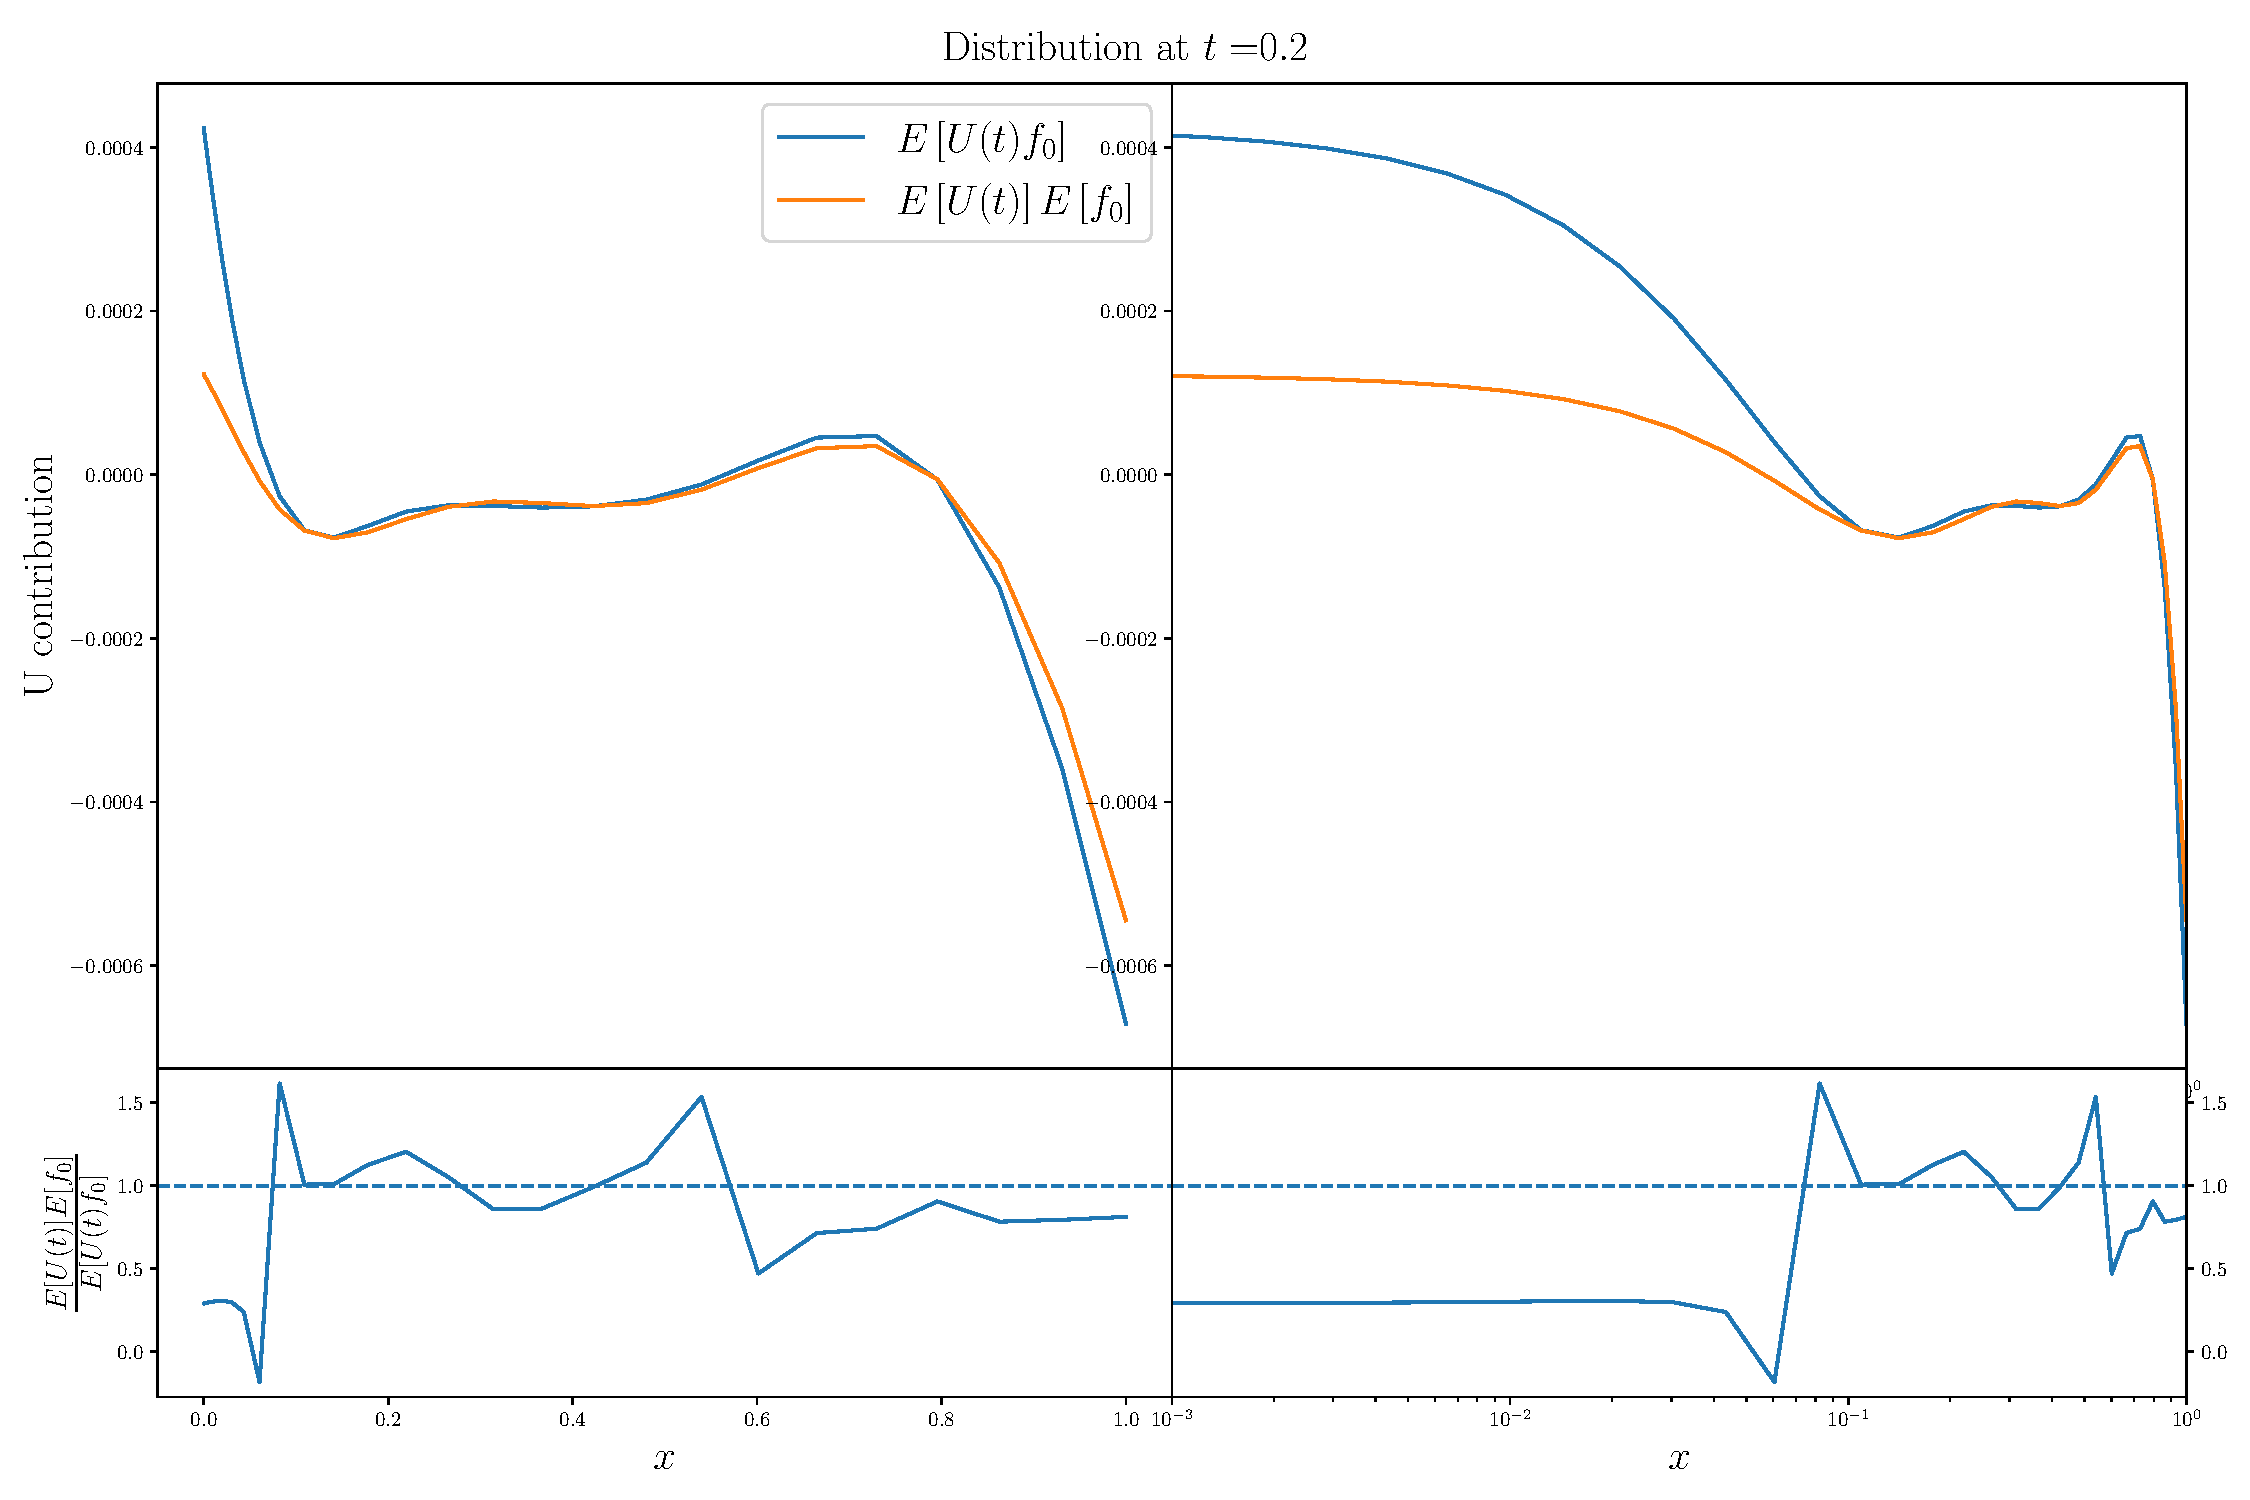
\includegraphics[width=0.65\textwidth]{plots/xT3_exp_val_eot.pdf}
  \caption{Expectation value of the product (blue) and product of the
  expectation value for the $U$ contribution. Plots obtained using $t_{\rm ref}
  = 30000$, while $f_0$ is an ensemble of networks at initialisation
  (\textit{i.e.} $\mathbb{E}[f_0]=0$). \ac{These plots will be modified (font
  size, etc...) to match the other figures.}}
\end{figure}
% ===================================


% L0 data
\begin{figure}[ht!]
    \centering
    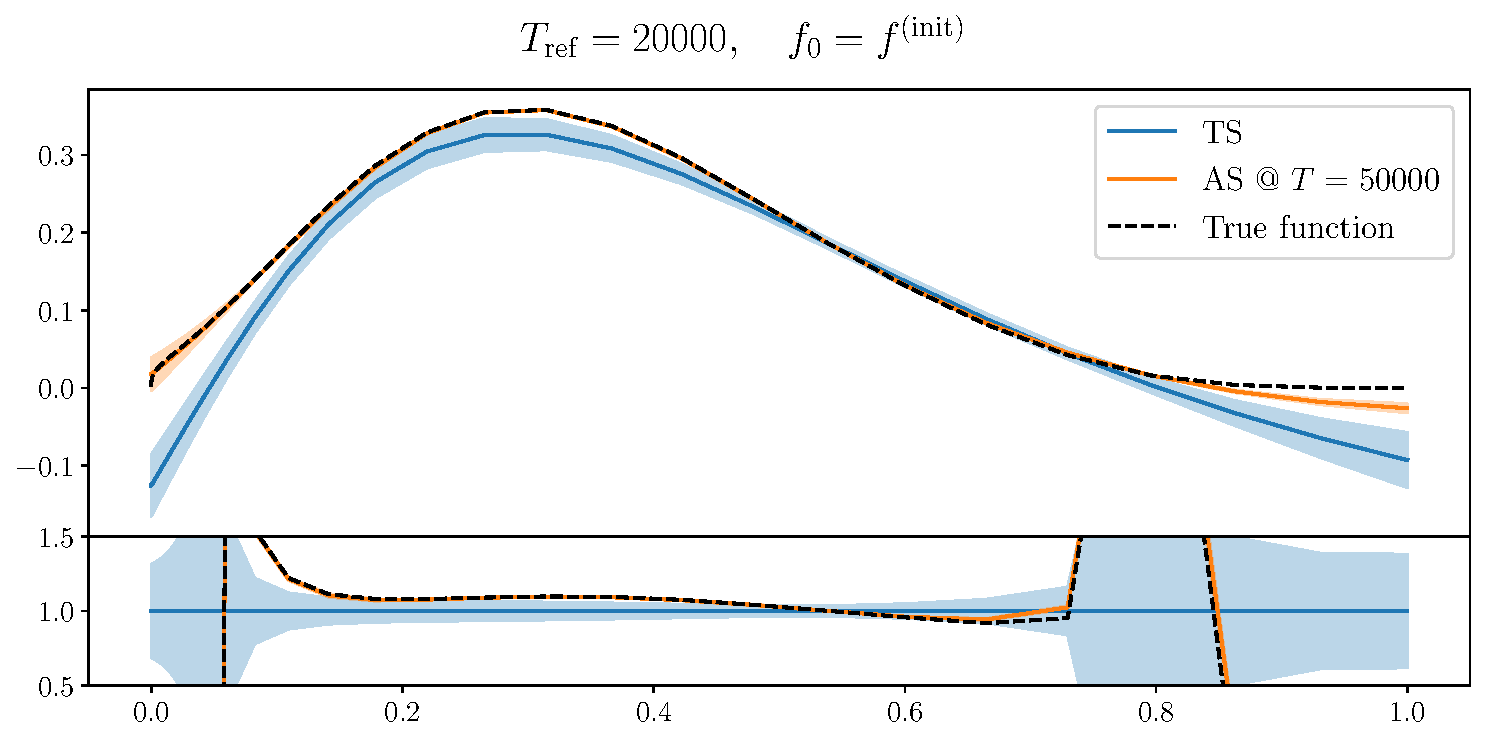
\includegraphics[width=0.48\textwidth]{plots/analytical_solution/pdf_plot_init_last_epoch_L0.pdf}
    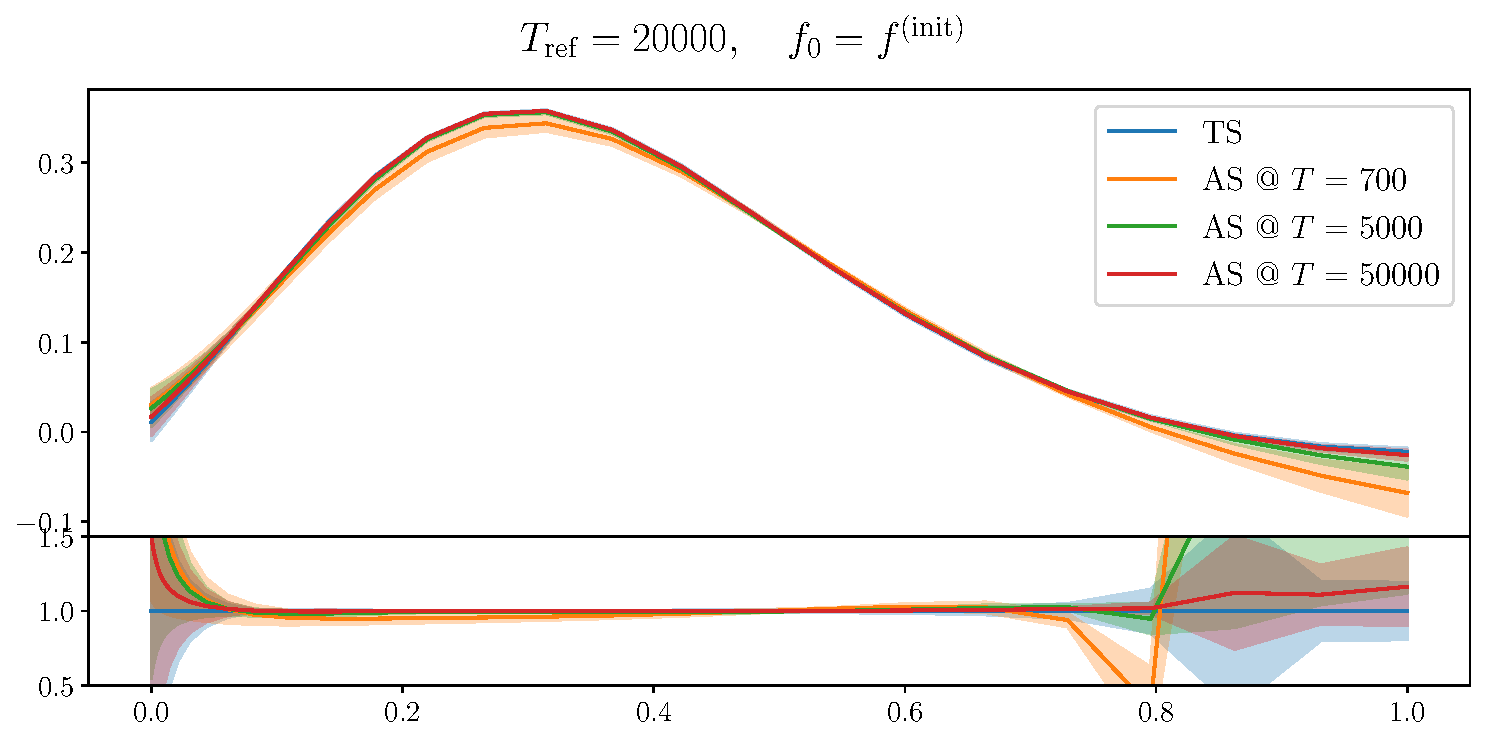
\includegraphics[width=0.48\textwidth]{plots/analytical_solution/pdf_plot_init_epochs_L0.pdf}
    \caption{Comparison of the trained solution at the end of training and
    the analytical solution using L0 data. In both panels, the
    frozen NTK is chosen at $T_{\rm ref} = 20000$ and the initial function $f_0$
    is a different ensemble of networks at initialisation. In the right panel,
    the analytical solution is evolved for $T_{\rm tot}$ epochs, while the left
    panel shows the same comparison for intermediate epochs.}
    \label{fig:xT3_analytical_init_L0}
  \end{figure}
  % ===================================
  \begin{figure}[ht!]
    \centering
    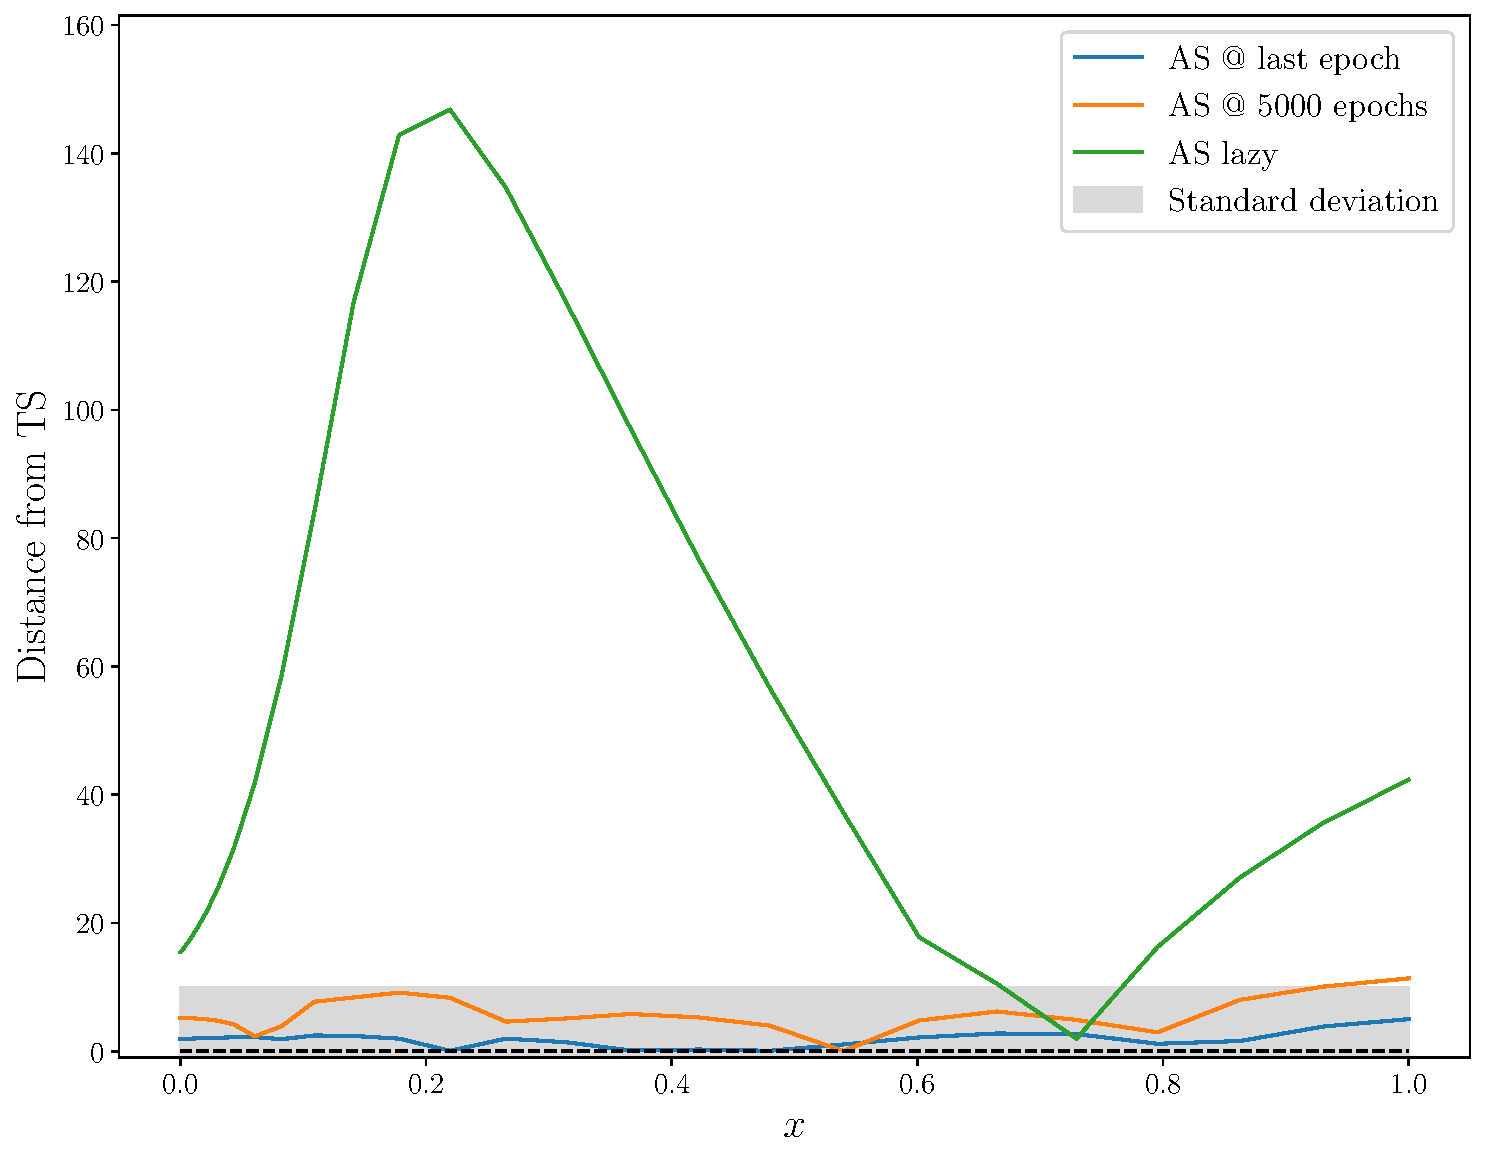
\includegraphics[width=0.48\textwidth]{plots/analytical_solution/distance_plot_L0.pdf}
    \caption{PDF distance, as defined in Ref.~\cite{NNPDF:2021njg}, with respect to
    the trained solution at the end of training and analytical
    solutions for various initial conditions and evolution epochs.}
    \label{fig:xT3_distance_L0}
  \end{figure}
  % ===================================

  % L2 data
\begin{figure}[ht!]
    \centering
    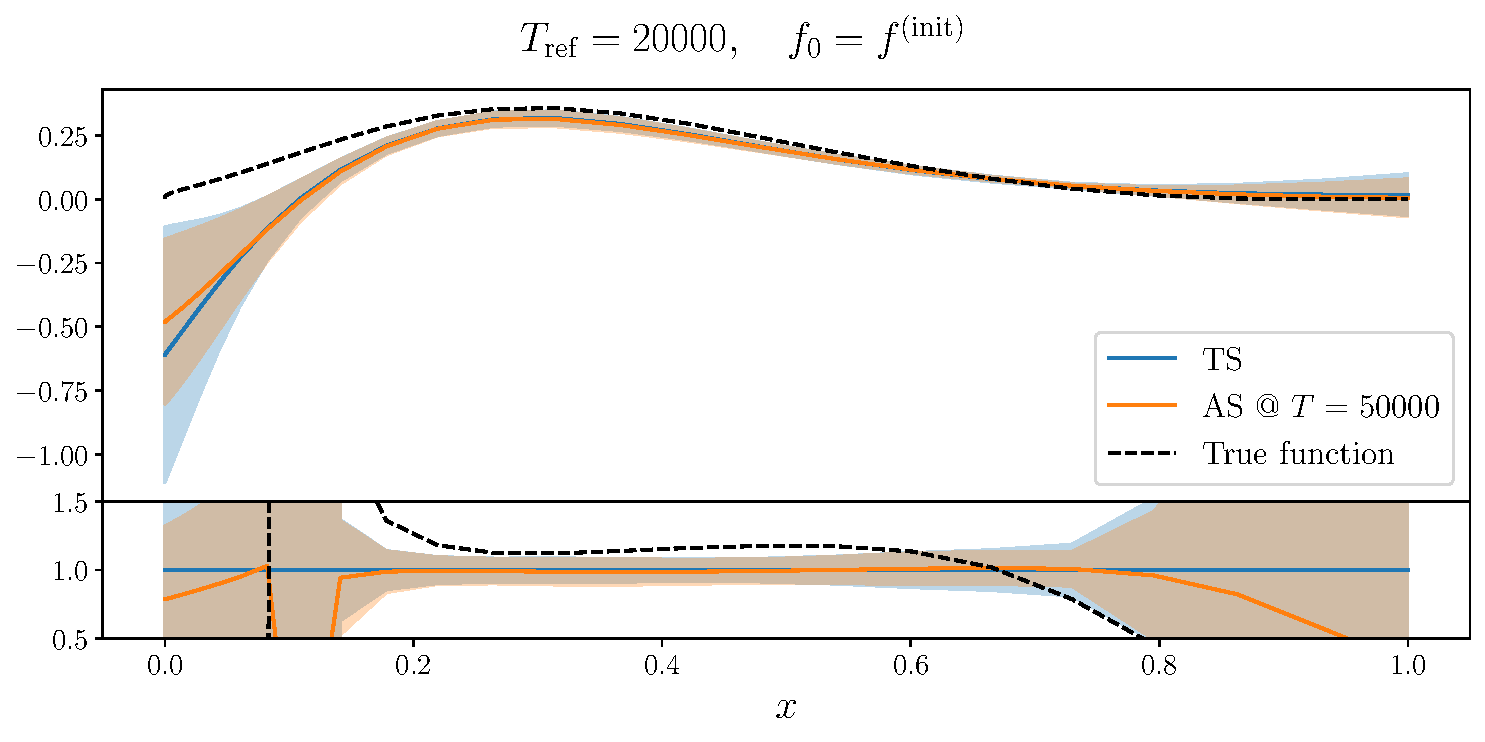
\includegraphics[width=0.48\textwidth]{plots/analytical_solution/pdf_plot_init_last_epoch_L2.pdf}
    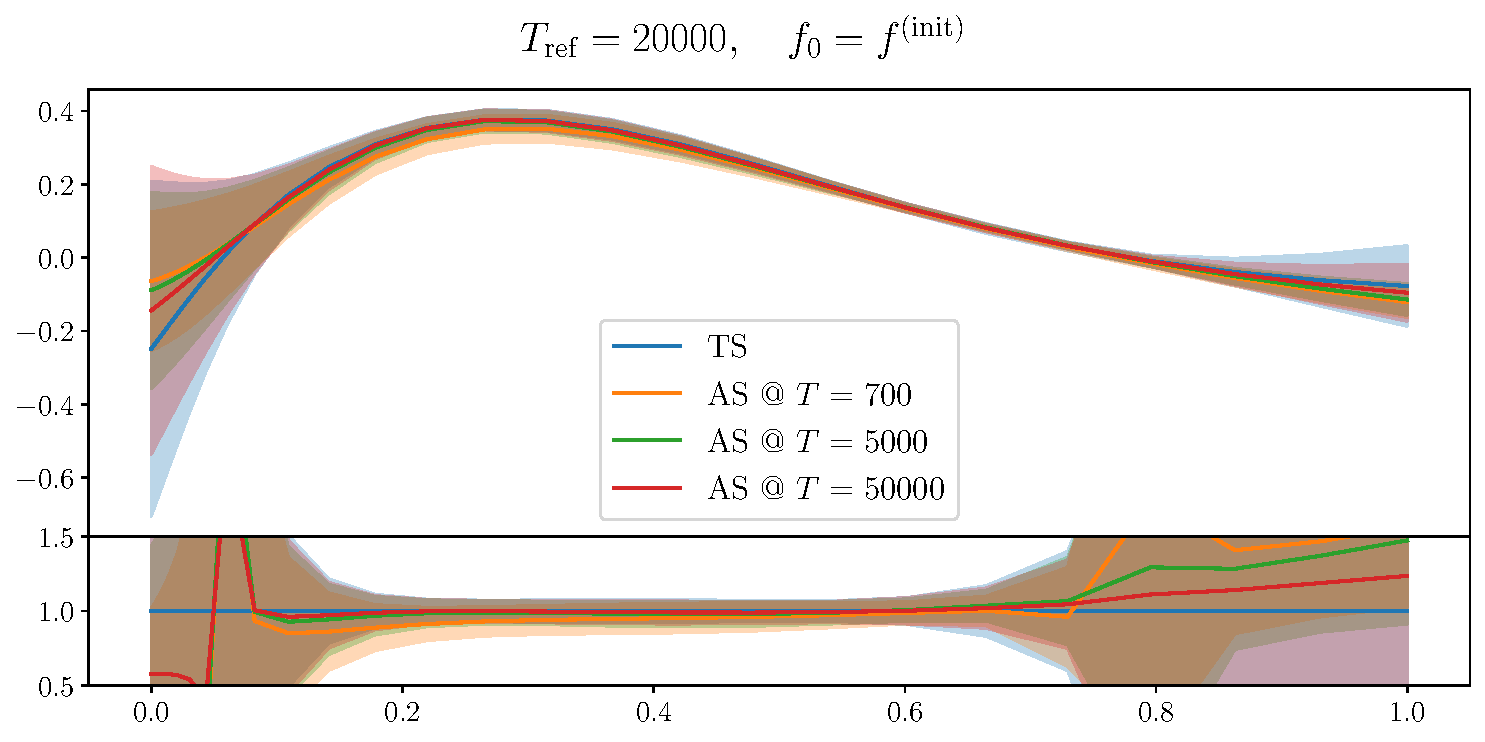
\includegraphics[width=0.48\textwidth]{plots/analytical_solution/pdf_plot_init_epochs_L2.pdf}
    \caption{Same as Fig.~\ref{fig:xT3_analytical_init_L0}, but using L2 data.}
    \label{fig:xT3_analytical_init_L2}
  \end{figure}
  % ===================================
  \begin{figure}[ht!]
    \centering
    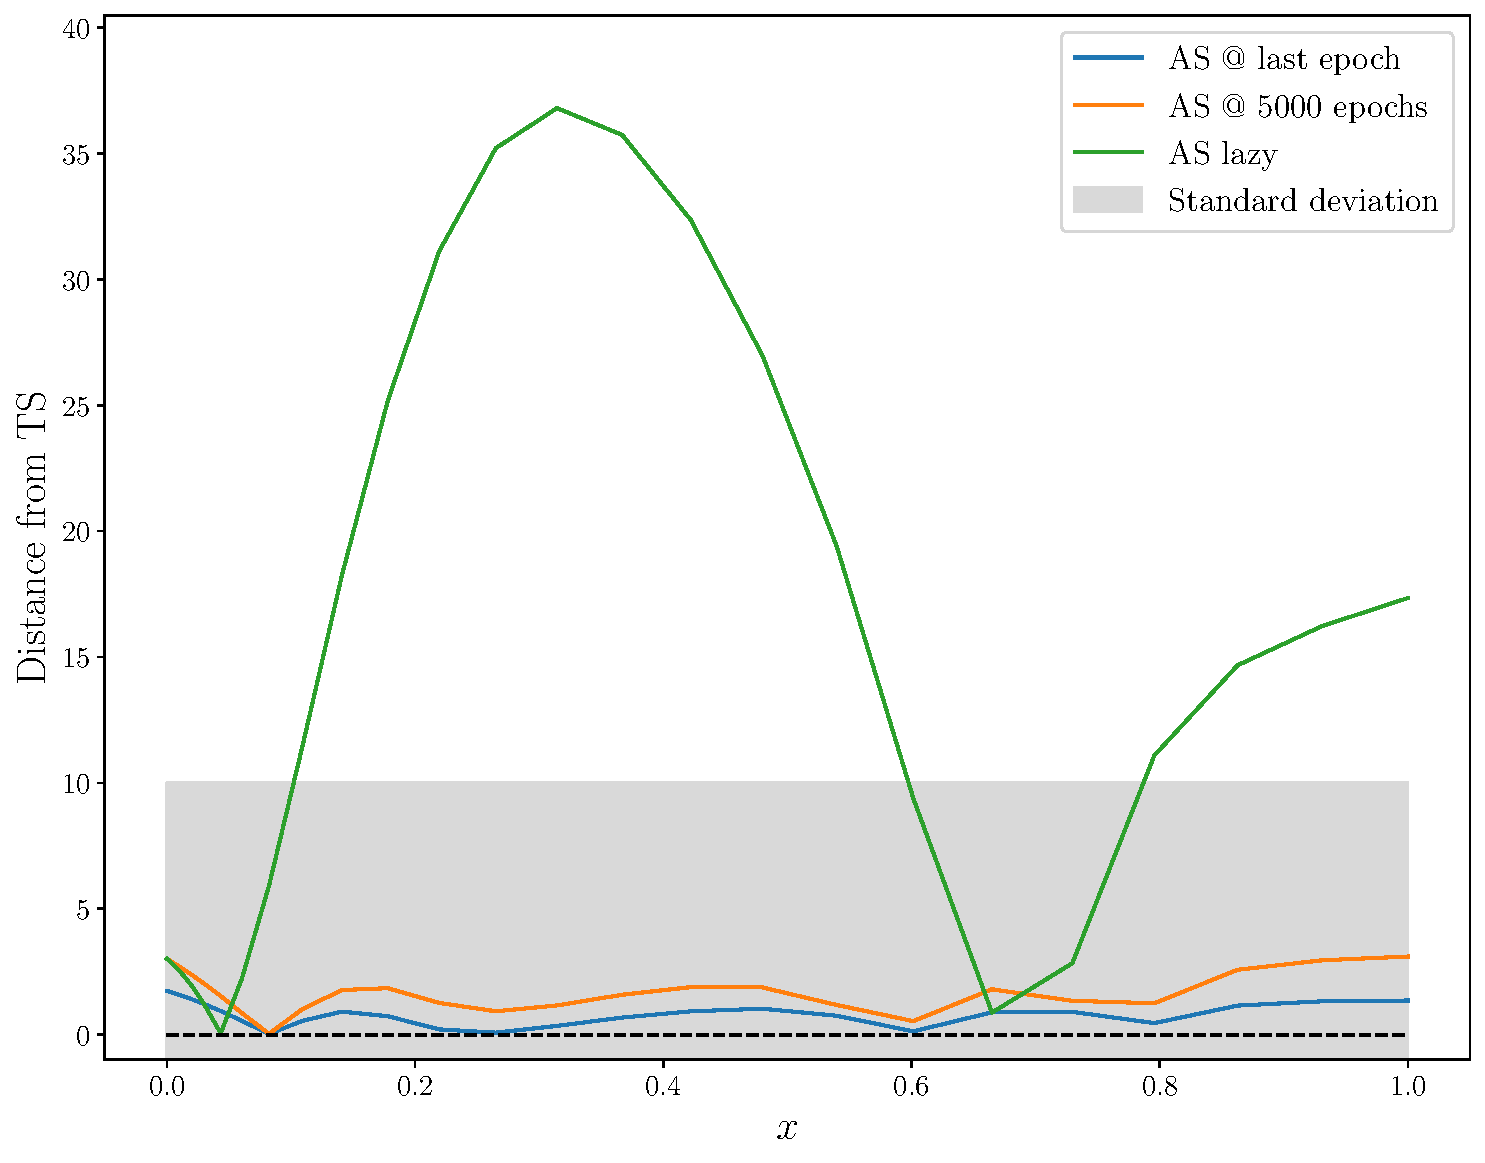
\includegraphics[width=0.48\textwidth]{plots/analytical_solution/distance_plot_L2.pdf}
    \caption{Same as Fig.~\ref{fig:xT3_distance_L0}, but using L2 data.}
    \label{fig:xT3_distance_L2}
  \end{figure}
  % ===================================


\begin{figure}[ht!]
    \centering
    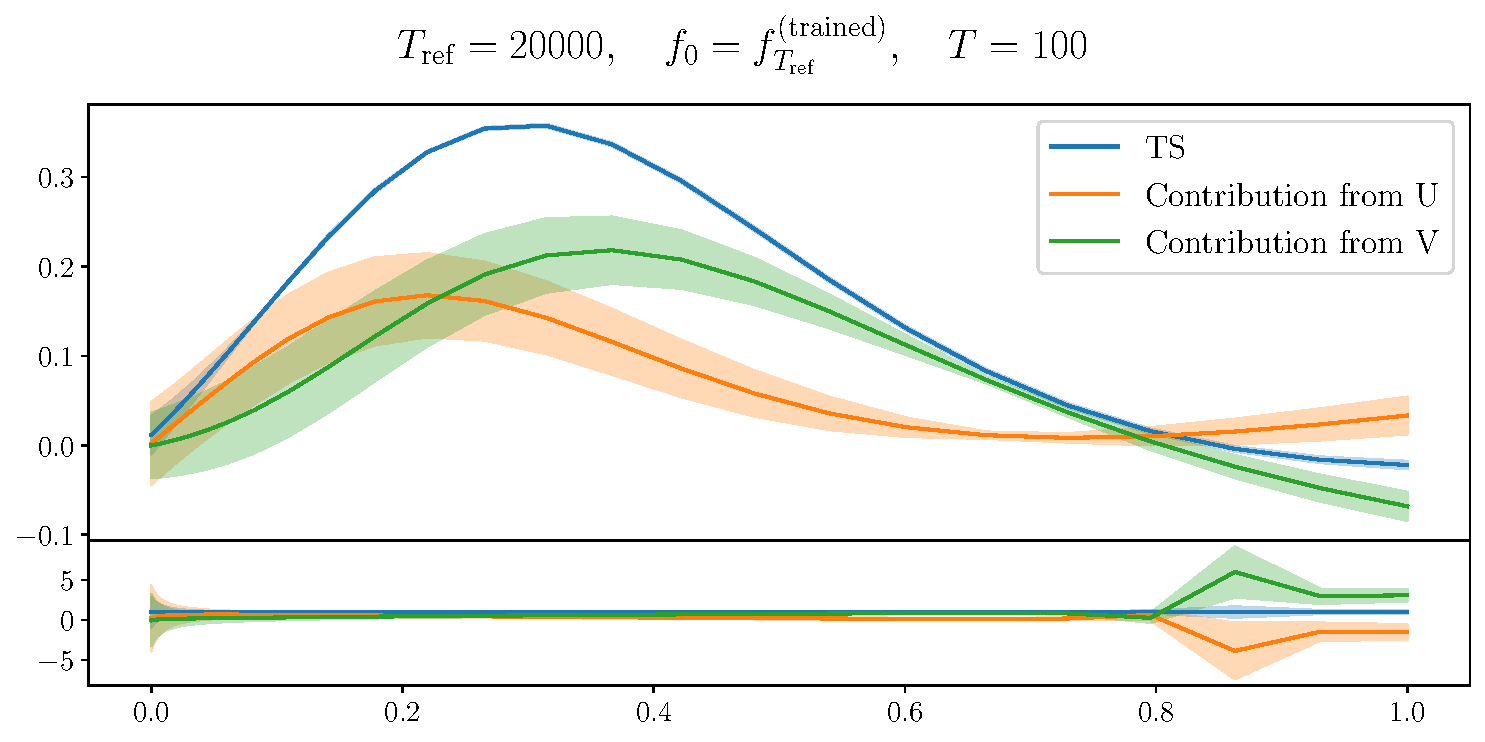
\includegraphics[width=0.45\textwidth]{plots/analytical_solution/pdf_plot_u_v_100_L0.pdf}
    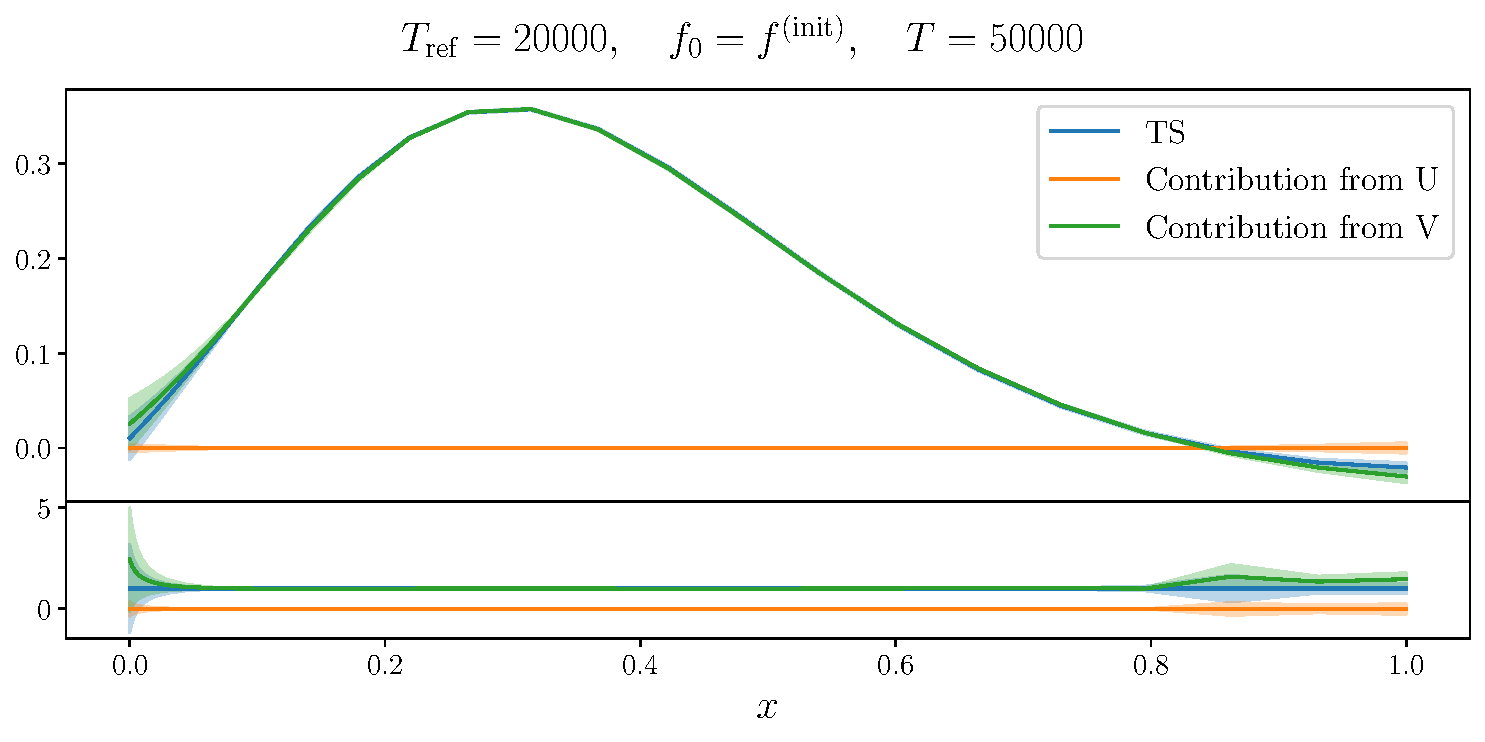
\includegraphics[width=0.45\textwidth]{plots/analytical_solution/pdf_plot_u_v_50000_L0.pdf}
    \caption{Contribution of the $U$ and $V$ terms to the analytical solution. The left
    panel shows this breakdown at early stages of the analytical training
    ($T=100$ epochs); the right panel shows the contributions at the end of
    training, as in Fig.~\ref{fig:xT3_analytical_init_L0}.}
    \label{fig:xT3_u_v_contributions_L0}
  \end{figure}
  % ===================================

  \begin{figure}[ht!]
    \centering
    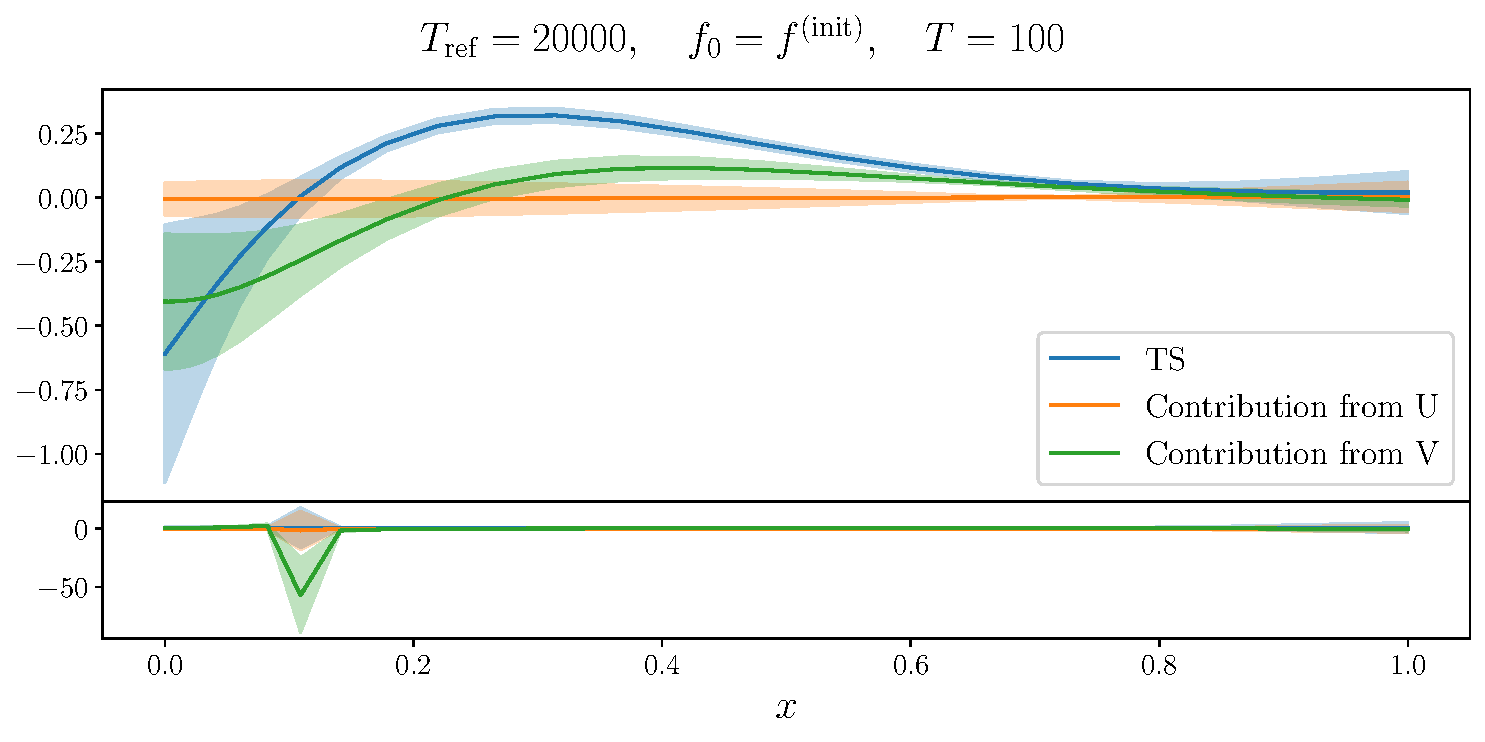
\includegraphics[width=0.45\textwidth]{plots/analytical_solution/pdf_plot_u_v_100_L2.pdf}
    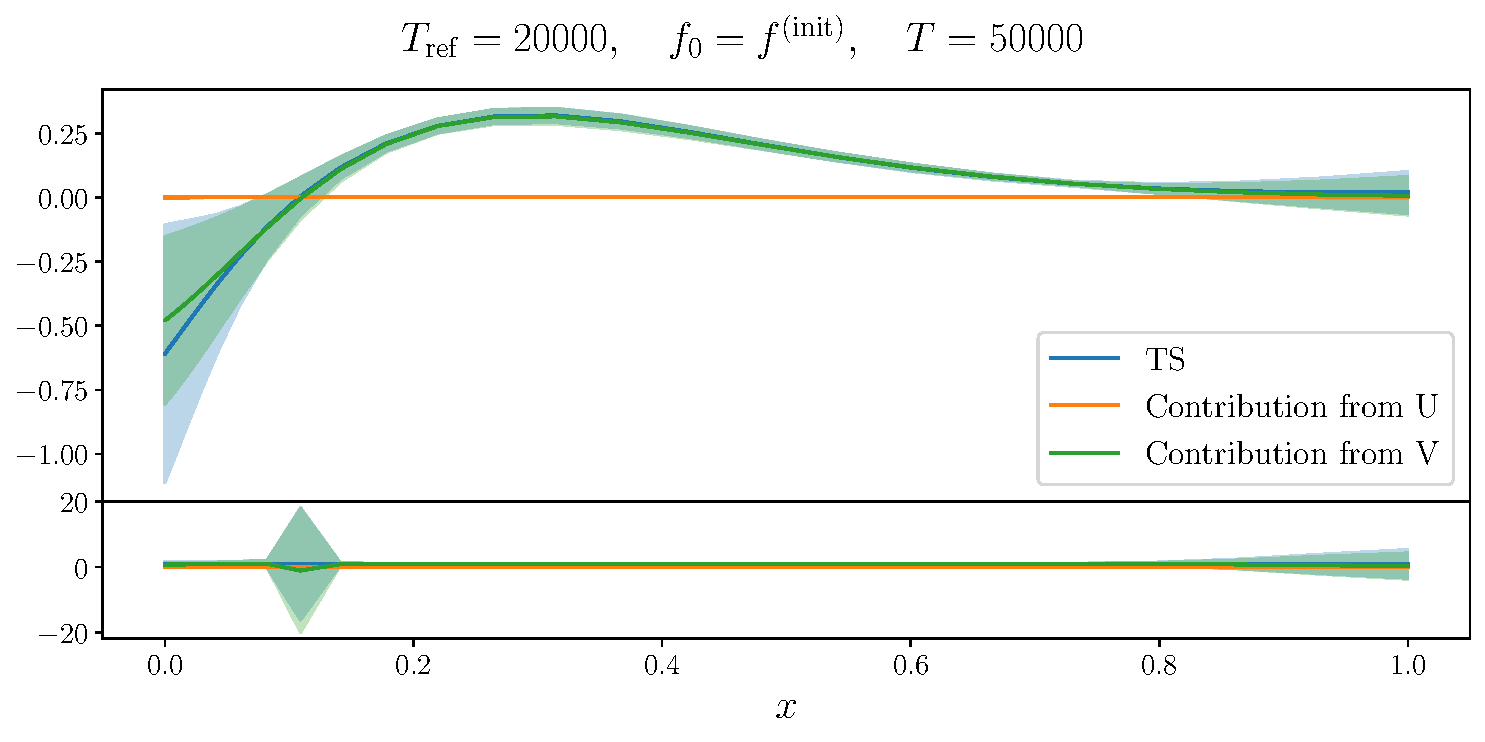
\includegraphics[width=0.45\textwidth]{plots/analytical_solution/pdf_plot_u_v_50000_L2.pdf}
    \caption{Same as Fig.~\ref{fig:xT3_u_v_contributions_L0}, but using L2 data.}
    \label{fig:xT3_u_v_contributions_L2}
  \end{figure}
  % ===================================


\FloatBarrier
